\documentclass{article}

\usepackage[brazil]{babel}

\usepackage{amsmath, amssymb}
\usepackage{graphicx}
\usepackage[colorlinks=true, allcolors=blue]{hyperref}

\usepackage{listings}
\lstset{
basicstyle=\small\ttfamily,
columns=flexible,
breaklines=true
}

\usepackage[section]{placeins}

\usepackage{tcolorbox}

\title{Relatório 05}
\author{Vinícius de Oliveira Peixoto Rodrigues (245294)}
\date{Março de 2023}

\begin{document}
\maketitle

\section{Introdução}


\section{Objetivos}

Este experimento tem como objetivo:

\begin{itemize}
    \item teste
\end{itemize}

\section{Metodologia}

\section{Resultados e Discussão}

\subsection*{Parte 1}

\begin{tcolorbox}
    Verifique quantos processos estão executando.
\end{tcolorbox}

\begin{lstlisting}
wifi@wifi-virtualbox:~$ sudo ps aux | grep quagga
quagga      3869  0.0  0.0   5136  3120 ?        Ss   13:34   0:00 /usr/lib/quagga/zebra -f confs/r1/zebra-r1.conf -d -i /tmp/zebra-r1.pid                                                                                           
quagga      3871  0.0  0.0   5216  3068 ?        Ss   13:34   0:00 /usr/lib/quagga/ospfd -f confs/r1/ospfd-r1.conf -d -i /tmp/ospf-r1.pid
quagga      3873  0.0  0.0   5140  3132 ?        Ss   13:34   0:00 /usr/lib/quagga/zebra -f confs/r2/zebra-r2.conf -d -i /tmp/zebra-r2.pid
quagga      3875  0.0  0.0   5212  2932 ?        Ss   13:34   0:00 /usr/lib/quagga/ospfd -f confs/r2/ospfd-r2.conf -d -i /tmp/ospf-r2.pid
quagga      3877  0.0  0.0   5140  3168 ?        Ss   13:34   0:00 /usr/lib/quagga/zebra -f confs/r3/zebra-r3.conf -d -i /tmp/zebra-r3.pid
quagga      3879  0.0  0.0   5212  1180 ?        Ss   13:34   0:00 /usr/lib/quagga/ospfd -f confs/r3/ospfd-r3.conf -d -i /tmp/ospf-r3.pid
quagga      3881  0.0  0.0   5144  3132 ?        Ss   13:34   0:00 /usr/lib/quagga/zebra -f confs/r4/zebra-r4.conf -d -i /tmp/zebra-r4.pid
quagga      3883  0.0  0.0   5212  1180 ?        Ss   13:34   0:00 /usr/lib/quagga/ospfd -f confs/r4/ospfd-r4.conf -d -i /tmp/ospf-r4.pid
quagga      3887  0.0  0.0   5140  3136 ?        Ss   13:34   0:00 /usr/lib/quagga/zebra -f confs/r5/zebra-r5.conf -d -i /tmp/zebra-r5.pid
quagga      3889  0.0  0.0   5216  1180 ?        Ss   13:34   0:00 /usr/lib/quagga/ospfd -f confs/r5/ospfd-r5.conf -d -i /tmp/ospf-r5.pid
quagga      3891  0.0  0.0   5136  3192 ?        Ss   13:34   0:00 /usr/lib/quagga/zebra -f confs/r6/zebra-r6.conf -d -i /tmp/zebra-r6.pid
quagga      3893  0.0  0.0   5212  1180 ?        Ss   13:34   0:00 /usr/lib/quagga/ospfd -f confs/r6/ospfd-r6.conf -d -i /tmp/ospf-r6.pid
wifi        4225  0.0  0.0   9032   740 pts/21   S+   14:20   0:00 grep --color=auto quagga
\end{lstlisting}

Está sendo executado um processo do \texttt{zebra} e um processo do \texttt{ospfd} para cada roteador (\texttt{r1,...,r6}).

\begin{tcolorbox}
    Com base nas informações contidas no Anexo desta Atividade (Quagga), o que estes processos representam?
\end{tcolorbox}

O \texttt{zebra} é um gerenciador de roteamento IP (que consegue
fazer a interface com o subsistema de rede do kernel), enquanto
o \texttt{ospfd} é a implementação do algoritmo OSPF em si. As
duas tarefas (interface com o sistema operacional/implementação
do gateway protocol) são separadas para desacoplamento e garantir
portabilidade.

\begin{tcolorbox}
    Existe conectividade entre x1 e y1? Comente.
\end{tcolorbox}

\begin{figure}[!htb]
\centering
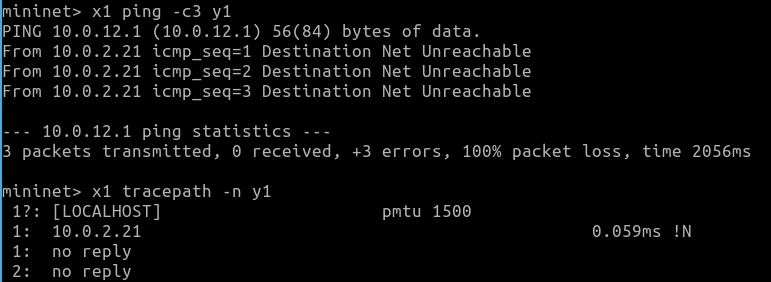
\includegraphics[width=\columnwidth]{images/p1_ping.png}
\caption{\texttt{ping} entre \texttt{x1} e \texttt{y1}.}
\end{figure}

Não há conectividade, e o traceroute demonstra que o pacote
para no roteador r1 (10.0.2.21), indicando que as tabelas de
roteamento não estão configuradas.

\subsection*{Parte 2}

\begin{tcolorbox}
    Quantas sub-redes existem na Figura 1? Informe os respectivos endereços de cada uma delas.
\end{tcolorbox}

Existem as seguintes subredes na configuração apresentada na imagem:

\begin{itemize}
    \item 10.0.2.0/23 (x1-eth1)
    \item 10.0.4.0/23 (r1-r2)
    \item 10.0.6.0/23 (r2-r3)
    \item 10.0.8.0/23 (r3-r4)
    \item 10.0.12.0/23 (r4-y1)
    \item 10.0.0.0/23 (r4, r6, r5)
    \item 10.0.10.0/23 (r5-r1)
\end{itemize}

\begin{tcolorbox}
    Qual das rotas difere das outras? Em quais aspectos?
\end{tcolorbox}

Na tabela de roteamento do roteador \texttt{r1}, encontramos o seguinte:

\begin{figure}[!htb]
\centering
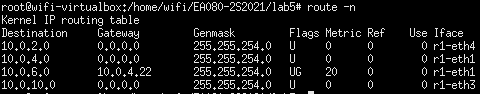
\includegraphics[width=\columnwidth]{images/p2_routes.png}
\caption{Tabela de roteamento de \texttt{r1}.}
\end{figure}

A diferença é a rota para \texttt{10.0.6.0/24}, que usa como
gateway o roteador \texttt{r2} (\texttt{10.0.4.22}) em vez
do \texttt{localhost} (\texttt{0.0.0.0}).

\FloatBarrier
\begin{figure}[!htb]
\centering
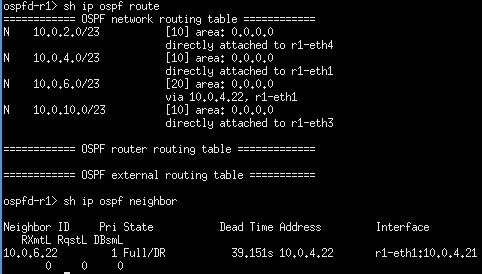
\includegraphics[width=\columnwidth]{images/p2_ospf.png}
\caption{Tabela de roteamento e os vizinhos de \texttt{r1}.}
\end{figure}
\FloatBarrier

\begin{tcolorbox}
    Quantos roteadores vizinhos o roteador \texttt{r1} possui?
    Qual o endereço da interface do(s) roteador(es) vizinho(s)?
    Por qual/quais interface(s) ele(s) está/estão conectado(s)?
\end{tcolorbox}

Somente um, o roteador \texttt{r2}, com endereço \texttt{10.0.6.22}
(\texttt{eth1} de \texttt{r2}) e conectado por meio da interface \texttt{10.0.4.21} (\texttt{eth1} de \texttt{r1}) a \texttt{10.0.4.22} (\texttt{eth2} de \texttt{r2}).

\begin{tcolorbox}
    Em que se assemelham as rotas vistas quando executado
    o comando \texttt{route -n} em \texttt{r1}, e as rotas
    mostradas pelo comando \texttt{sh ip ospf route}?
\end{tcolorbox}

As rotas do comando \texttt{route} são listadas no Quagga como
\texttt{OSPF network routing table}, enquanto as rotas externas
do OSPF são listadas como \texttt{OSPF external routing table}.

\begin{tcolorbox}
    Com base na topologia da Fig. 1, por qual roteador foi
    anunciada a rota que difere das outras?
\end{tcolorbox}

Foi anunciada por \texttt{r2}, visto que ele é usado como gateway.

\end{document}
